\documentclass[12pt,letterpaper,english,bibliography=totocnumbered, abstract=on]{scrartcl}

\usepackage[page,toc,titletoc,title]{appendix}


\usepackage{indentfirst}
\usepackage[titletoc]{appendix}
%\usepackage{fullpage}
%\usepackage{subfiles}
\usepackage[T1]{fontenc}
\usepackage[latin9]{inputenc}
\usepackage{color}
\usepackage{babel}
\usepackage{verbatim}
\usepackage[unicode=true,pdfusetitle,
bookmarks=true,bookmarksnumbered=false,bookmarksopen=false,
breaklinks=true,pdfborder={0 0 0},pdfborderstyle={},backref=false,colorlinks=true]
{hyperref}
\hypersetup{linkcolor=blue,citecolor=blue,urlcolor=blue}

\usepackage{booktabs}
\usepackage{multirow}
\usepackage{adjustbox}
\usepackage{threeparttable}
\usepackage[table]{xcolor}
\usepackage{csquotes}
\usepackage{soul} % for hiliting text: \hl

\usepackage[backend=biber, sorting=none]{biblatex}
\addbibresource{CRB.bib}
\addbibresource{extra.bib}

\usepackage{pdfpages}
\usepackage{float} % Allows use of H to place floats

\usepackage{pgfgantt}

\usepackage{framed}
\usepackage{todonotes}

\usepackage{gensymb}

% Prevent page breaks within paragraphs
% https://tex.stackexchange.com/questions/21983/how-to-avoid-page-breaks-inside-paragraphs
\widowpenalties 1 10000


\begin{document}

\titlehead{Final Report: USFS 20-DG-11052021-227}

\title{Improving Coconut Rhinoceros Beetle Breeding Site Detection Using Harmonic Radar}

\author{Aubrey Moore PhD\\University of Guam College of Natural and Applied Sciences}

%\date{January 30, 2023}

\maketitle

\begin{description}
	\item[Federal ID] 20-DG-11052021-227
	\item[Reporting period] 2020-06-17 through 2022-12-31
\end{description}


\begin{footnotesize}	
	\url{https://github.com/aubreymoore/Harmonic-Radar/raw/master/final-report-202212/final-report-202212.pdf}
\end{footnotesize}

\clearpage

\tableofcontents

\clearpage


\section{Using Harmonic Radar to Detect CRB Breeding Sites}

Effective control of CRB requires location and destruction of larval breeding sites which my occur anywhere were there is an accumulation of decaying plant material. Previously, we successfully tracked radio-tagged CRB adults to find cryptic breeding sites \cite{moore_judas_2017-1}. But high cost of radio transmitters (about \$200 each) and limited battery capacity make this method too expensive for regular use. 

We suggest that harmonic radar tags may be a cost-effective replacement for miniaturized radio transmitters. Harmonic radar tags do not require a battery, are very inexpensive (about \$4 per tag) and have unlimited shelf and field life. 

US Forest Service funded a field test of this idea based on a small grant proposal  attached as Appendix \ref{appA}. We also published the idea as a journal article \cite{mooreProposalDetectingCoconut2022} attached as Appendix \ref{appB}.

\newpage
\section{Field Test}

In July 2022, Dr. Matt Siderhurst, from Eastern Mennonite University, Virginia and two of his students, Skylar List and and Theodore Yoder, travelled to Guam to collaborate with us on Guam to field test the idea of tracking beetles with miniature harmonic radar tags attached to them. We were also assisted by Michael Jordan, US Forest Service and my technician, Christian Cayanan.

We used an Open Science Framework (OSF) project \cite{Moore_Yoder_Cayanan_List_2023} to document this field trial. \href{https://osf.io/esnc7/}{Details are available online}. The following subsections summarize what we did and what we learned.

\subsection{Materials and Methods}

\paragraph{Harmonic radar tags}

We fabricated dipole harmonic radar tags by attaching antennae to Schottky diodes (RECCO AB, Liding�, Sweden). Two 8 cm lengths of super-elastic nitinol wire (0.076 mm diameter, McMaster-Carr, Aurora, OH, USA) were attached to each diode with UV-activated adhesive (Bondic, Niagara Falls, NY, USA), so that each wire touched one of the diode contacts while avoiding the opposite diode contact and the other wire. Electrical connections between the wires and diode contacts were secured using conductive silver paint (GC Electronics, Rockford, IL, USA). Radar tags were glued to the top of the pronotum of each test beetle using UV-activated adhesive.

\paragraph{Insects}

CRB adults were collected from pheromone traps at the Leo Palace Resort on DATE.  These insects were held in moist coir REF and were fed banana slices.

\paragraph{Tagged insect releases}

About an hour before sunset, tagged beetles were placed in a 10 cm deep layer of damp coir at the bottom of a large plastic garbage container. Most beetles readily flew out of the container within an hour after sunset. Early the next morning, beetles remaining in the coir were counted.

A total of 27 tagged beetles were released at the University of Guam Yigo Experiment Station on July 7 and 11 and 39 beetles were released in Yona on July 12.

\paragraph{Search for tagged insects}

During days following tagged beetle releases, we performed surveys using three hand-held harmonic radar devices (RECCO AB, Liding�, Sweden) designed for finding avalanche victims. Searchers monitored audio output from the radar devices using headphones and recorded their search paths using a smart phone app REF.

Surveys were conducted at Yigo on July 8, 12 and 15 and at Yona on July 13 and 15.

\subsection{Results and Discussion}

About two-thirds of the tagged beetles flew out of the large plastic garbage containers at release sites (Table \ref{table1}). However, no tagged beetles were detected during 5 harmonic radar surveys conducted following release.

\begin{table}[!ht]
	\centering
	\caption{Numbers of beetles which flew out of and remained in large garbage containers at release sites.}
	\label{table1}
	\begin{tabular}{lcccc}
		\hline
		site & date & total & flew & did not fly \\ \hline
		Yigo & July 7 & 32 & 12 & 20 \\
		Yigo & July 11 & 30 & 19 & 11 \\
		Yona & July 12 & 39 & 33 & 5 \\ \hline
		~ & ~ & 101 & 64 & 36 \\ \hline
	\end{tabular}
\end{table}

\paragraph{Failure analysis}

Examination of beetles which failed to fly out of the large garbage containers at release sites showed a problem with attachment of antennae to the diodes. 
Sixty-one percent (22 of the 36) beetles which did not fly had damaged tags: 22 had one or more detached antenna wires and one had a detached diode (Table \ref{table2}).

Apparently, the silver conductive paint and UV-cured glue did not create a physical bond strong enough for this application. Electrical connectivity may also be a problem. 

We are now attempting to solve this technical problem by attaching antennae wires by soldering them to diodes under a microscope.

We purchased precision soldering equipment for this. However, our first attempt failed. Getting solder to "wet" nitinol wire, made from an allow of nickel and tin, is difficult because of oxides on the surface of the wire need to be removed. We have ordered a special soldering kit specifically designed for nitinol and will give this a try when it arrives.

\begin{table}[!ht]
	\centering
	\caption{Status of harmonic radar tags attached to beetles remaining in release containers.}
	\label{table2}
	\begin{tabular}{lcccc}
		\hline
		site & date & total & wire(s) detached & diode detached \\ \hline
		Yigo & July 7 & 20 & 6 & 0 \\
		Yigo & July 11 & 11 & 11 & 1 \\
		Yona & July 12 & 5 & 5 & 0 \\ \hline
		~ & ~ & 36 & 22 & 1 \\ \hline
	\end{tabular}
\end{table}

\section{Ancillary experiments}

\subsection{Expt.1: Maximum detection distances for each of the 3 RECCO transceivers we used}
Please see Jupyter notebook in Appendix \ref{exp1}.

\subsubsection{Expt. 2: Maximum detection distances for single and double tagged CRB}
Please see Jupyter notebook in Appendix \ref{exp2}.

\subsection{Expt. 3: Attenuation of maximum detection distances when targets are buried in coir}
Please see Jupyter notebook in Appendix \ref{exp3}.

\printbibliography

\newpage
\begin{appendices}

\section{Grant Proposal}
Please see next page.
\label{appA}
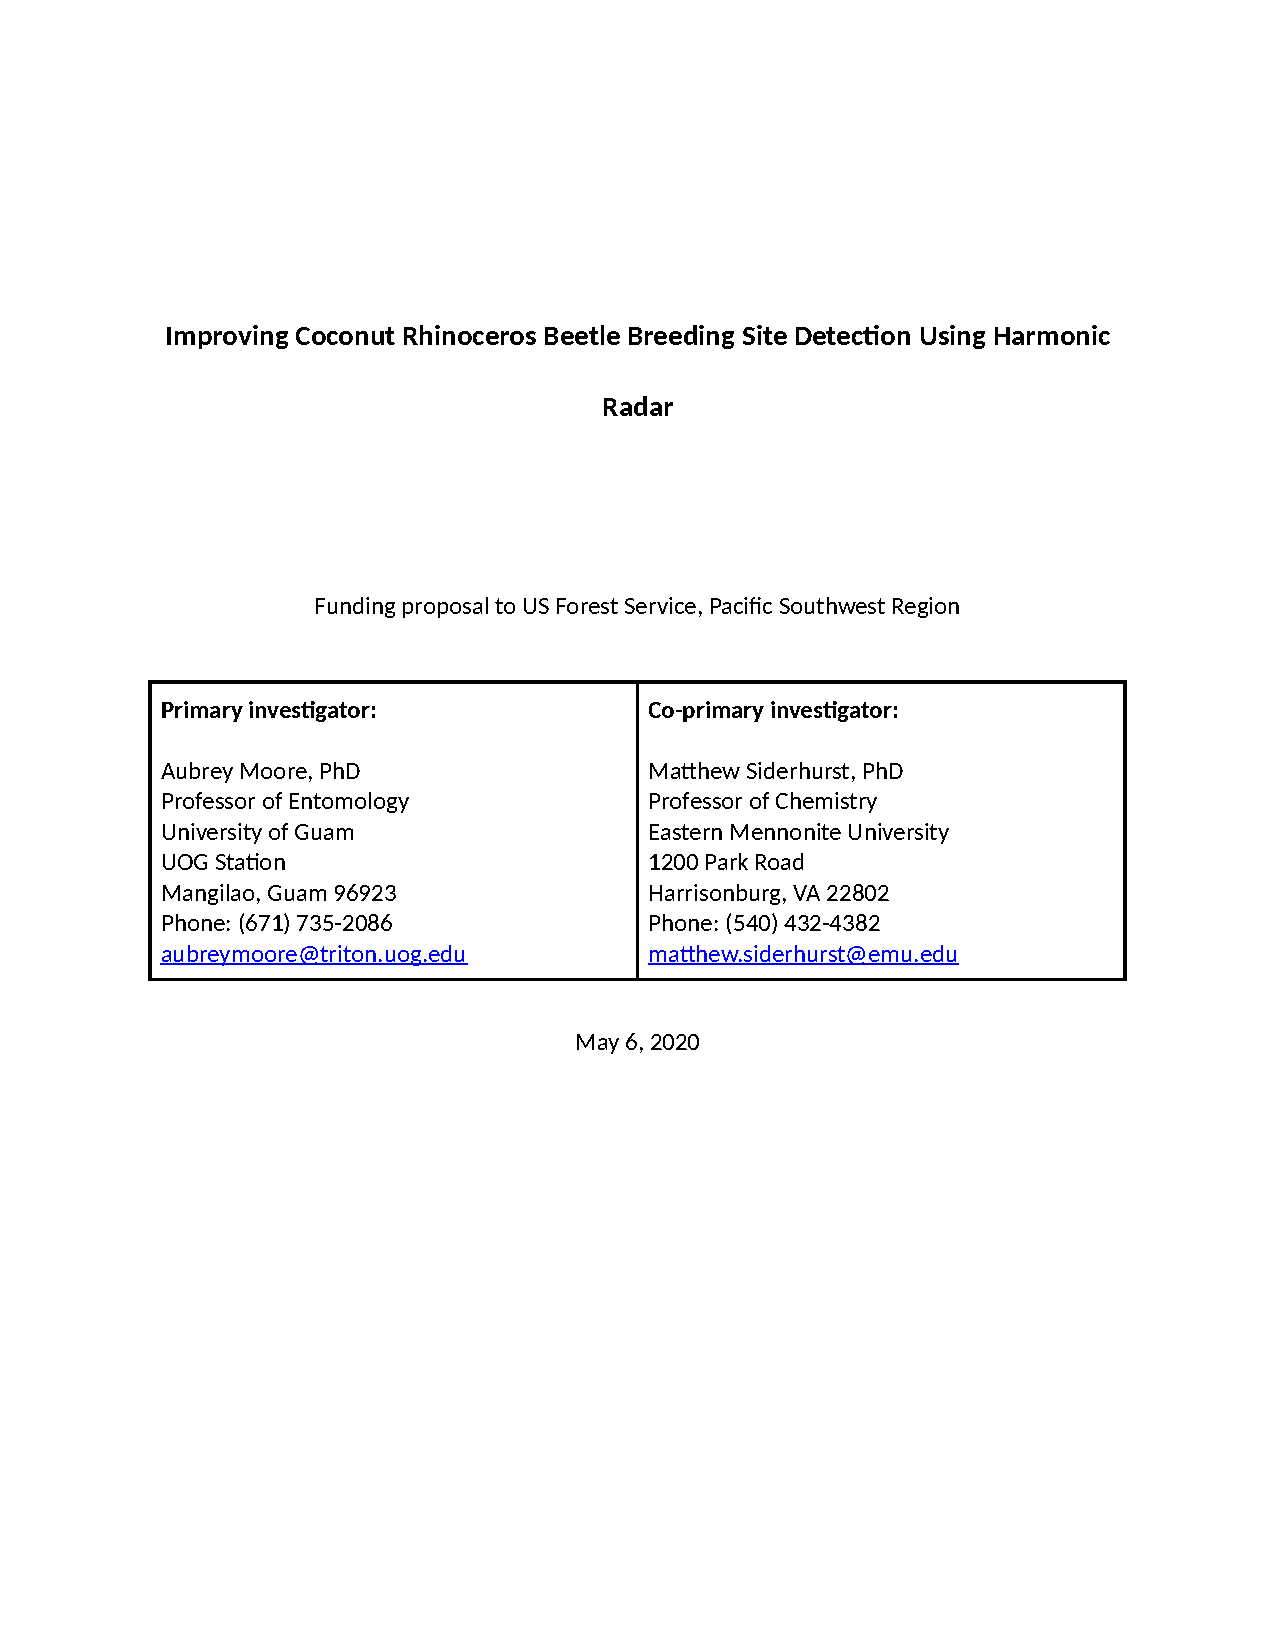
\includepdf[pages=-]{../USFS-harmonic-radar-proposal.pdf}

\newpage
\section{Journal Article}
\label{appB}
Please see next page.
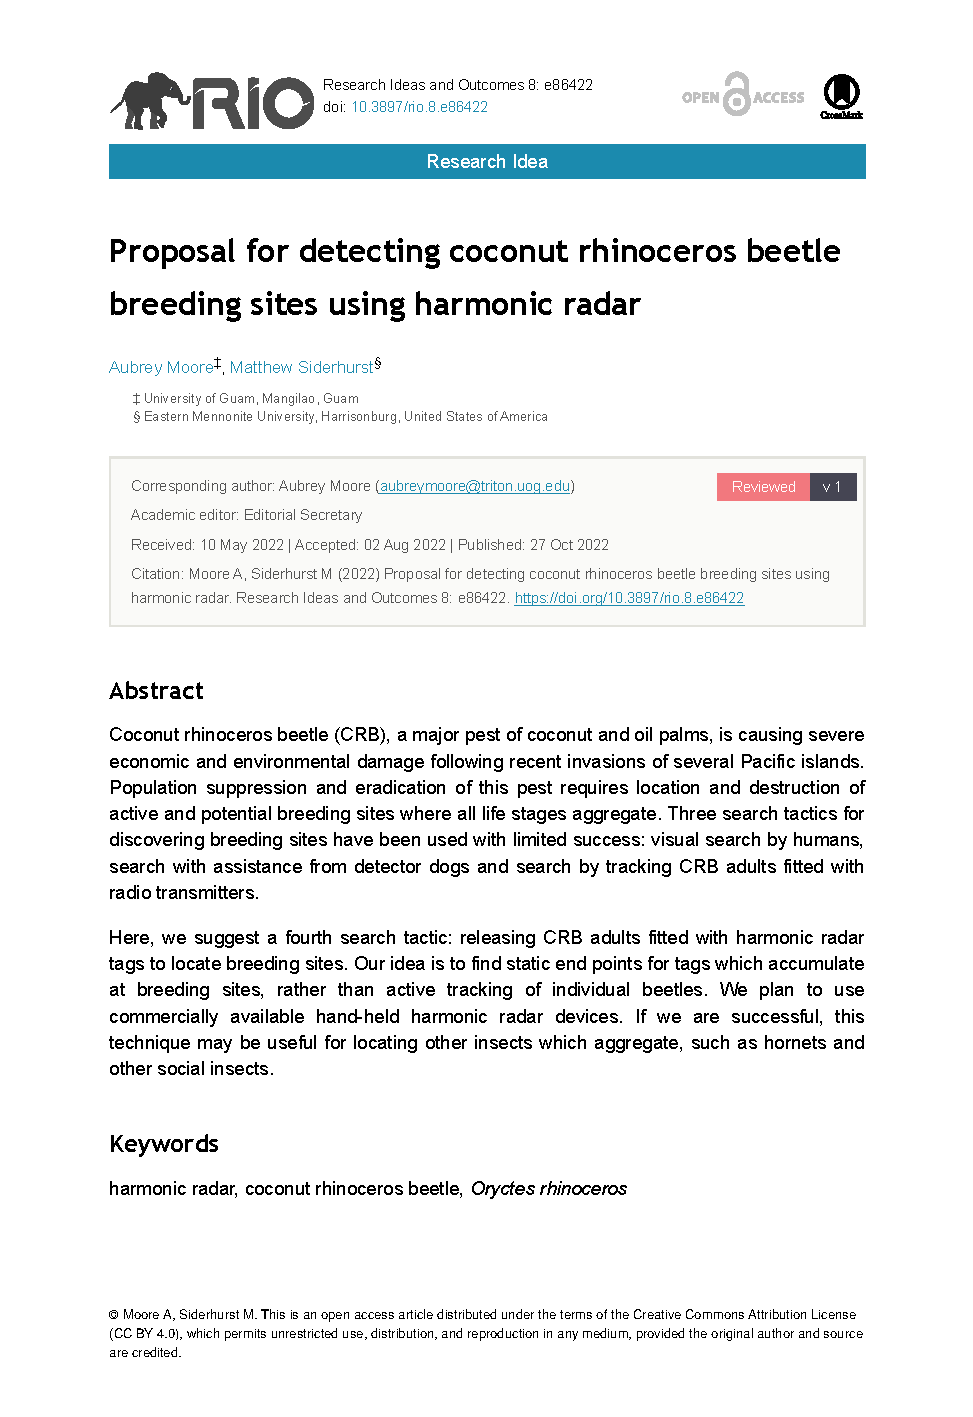
\includepdf[pages=-]{../Moore-and-Siderhurst2022.pdf}

\newpage
\section{Progress Report 4}
\label{appC}
Please see next page.
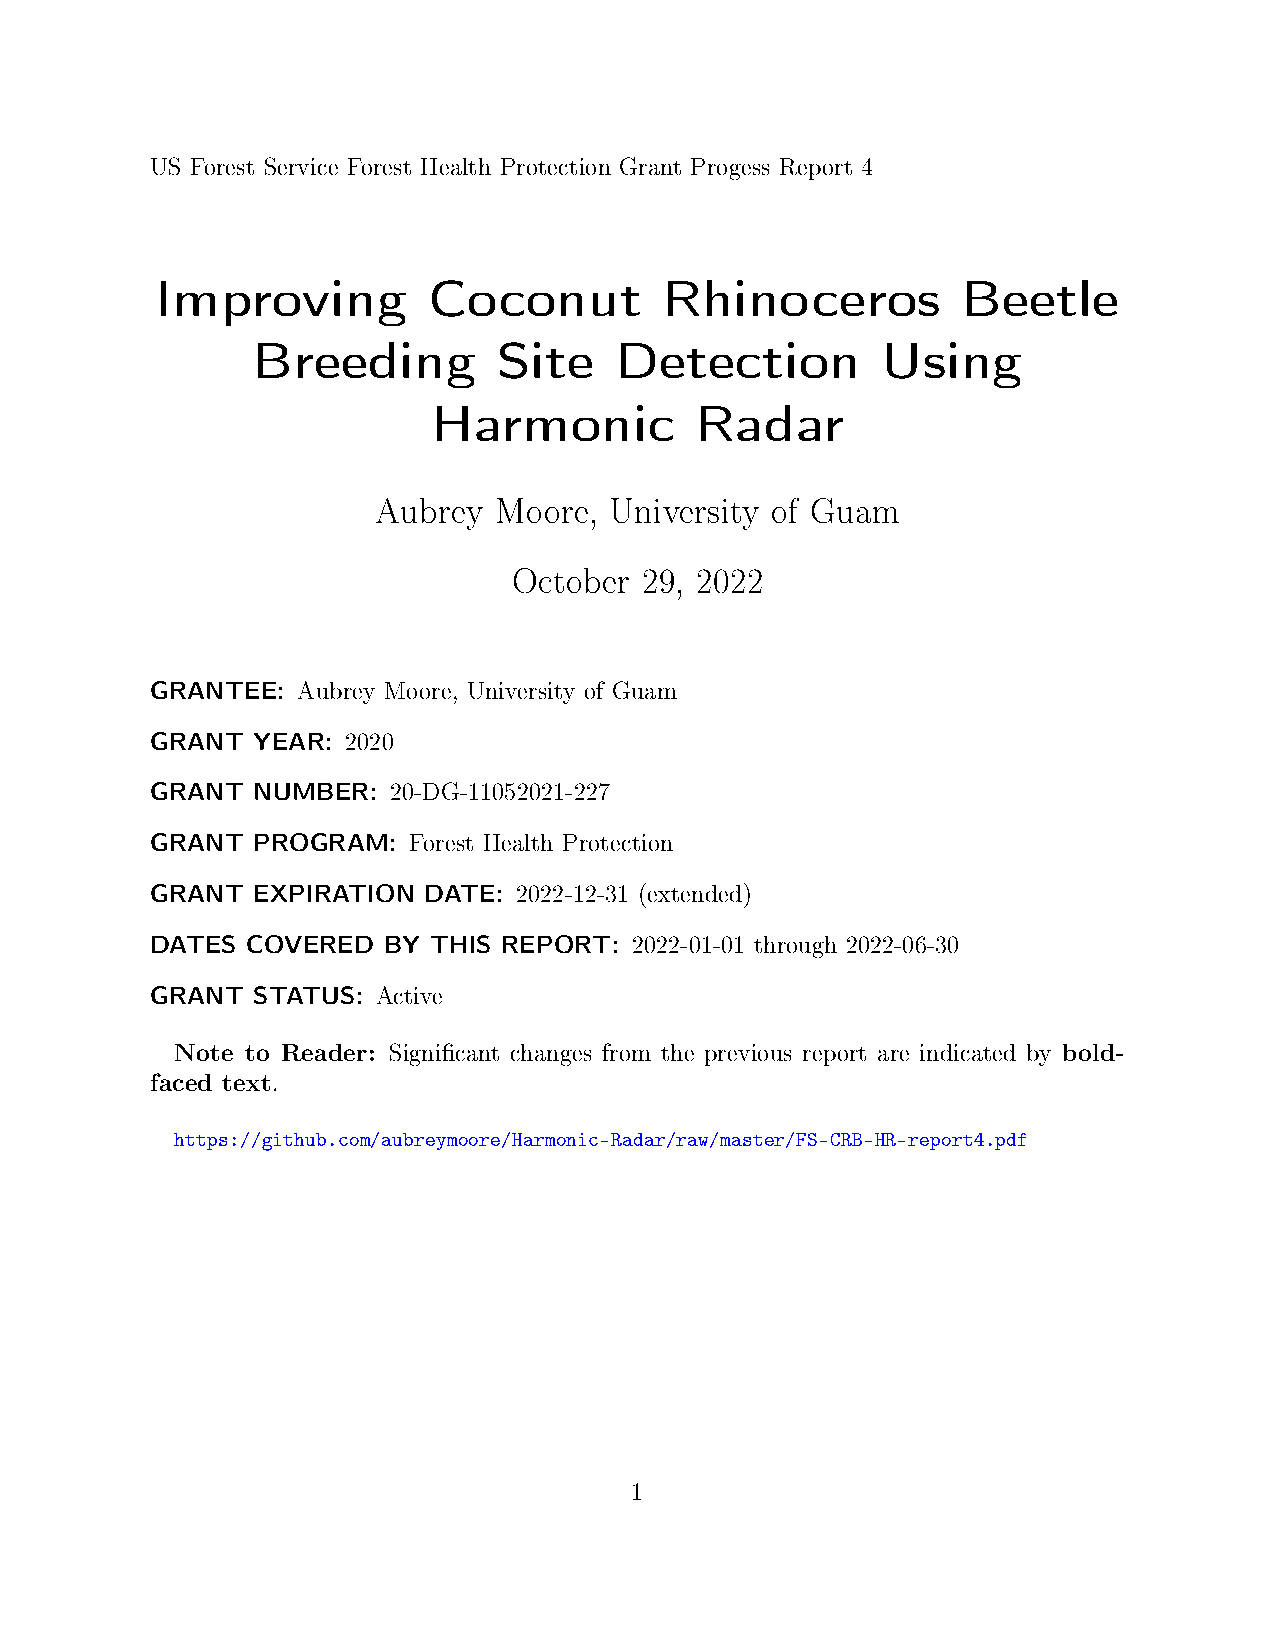
\includepdf[pages=-]{../FS-CRB-HR-report4.pdf}

\newpage
\section{Jupyter Notebook for Experiment 1: Maximum detection distances for each of the 3 RECCO transceivers we used}
\label{exp1}
Please see next page.
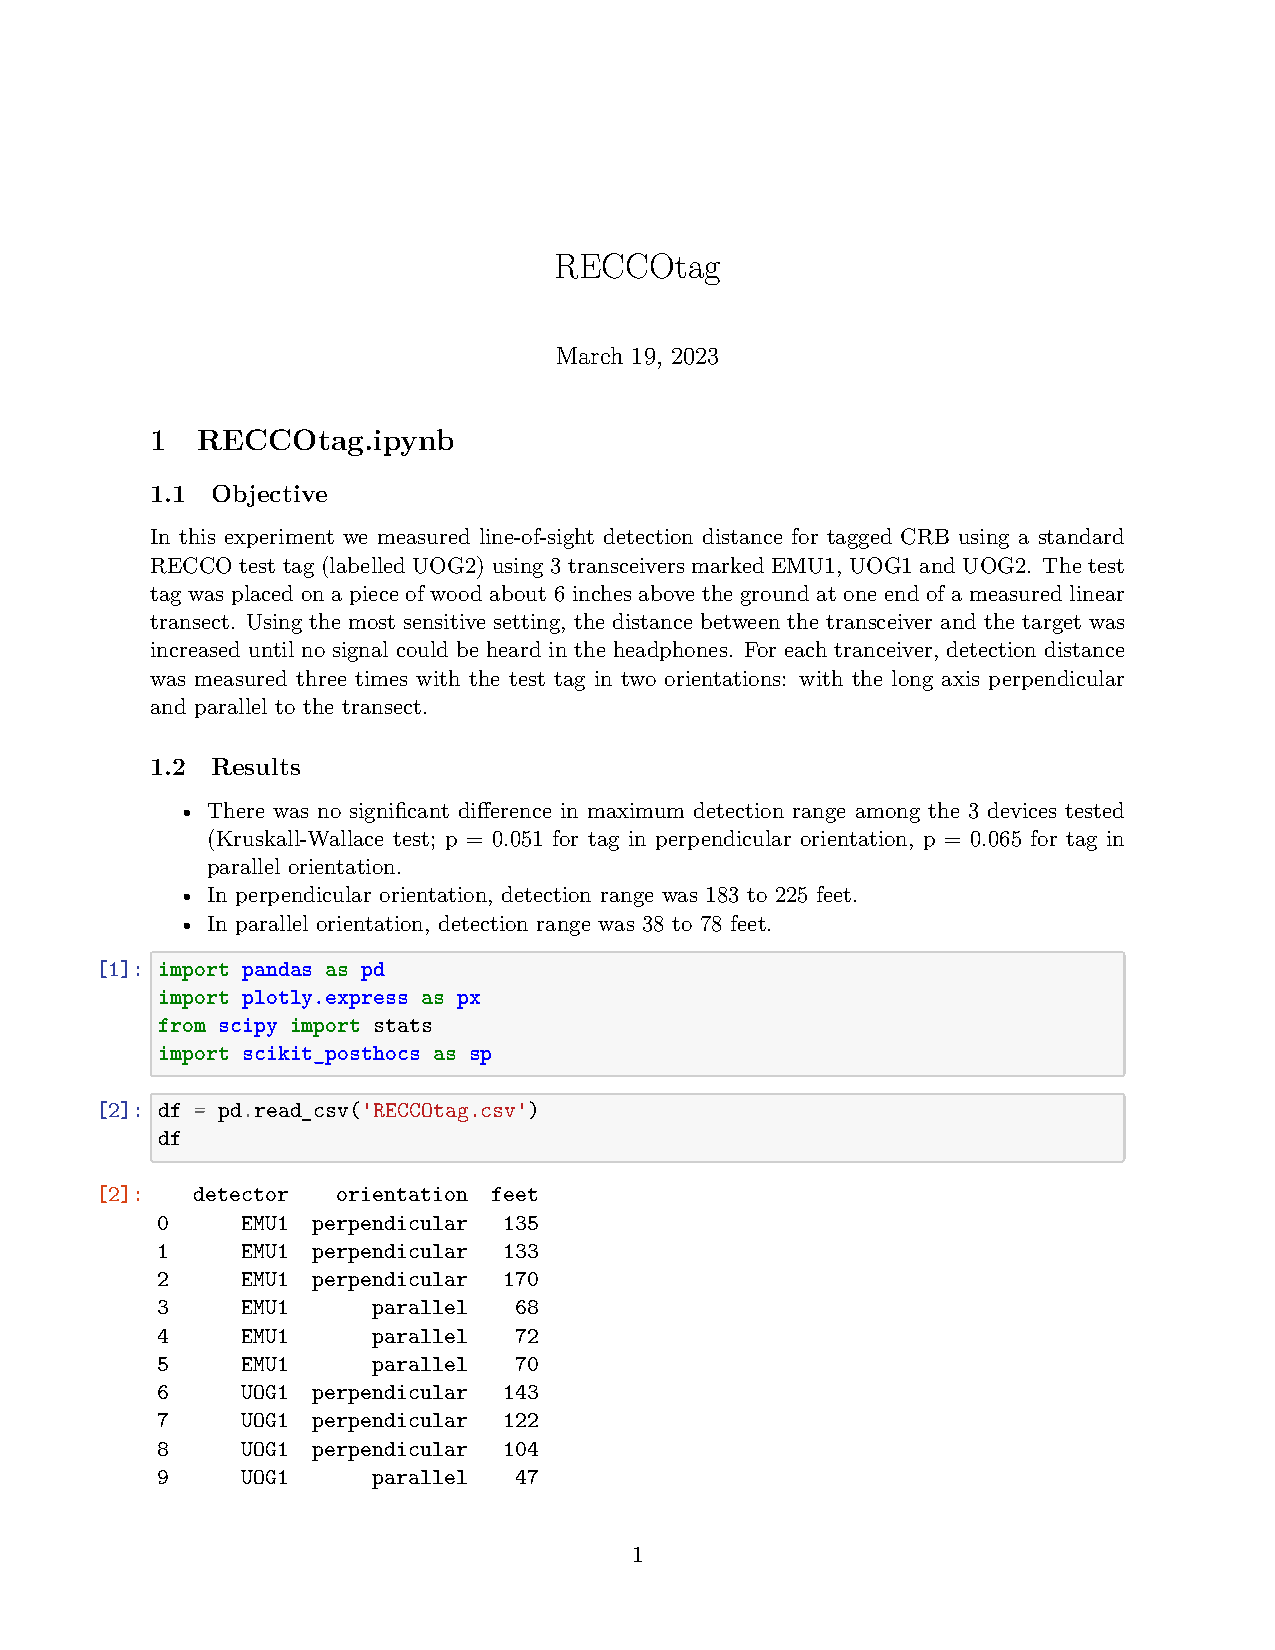
\includepdf[pages=-]{../experiments/detection-range/RECCOtag.pdf}

\newpage
\section{Jupyter Notebook for Experiment 2: Maximum detection distances for single and double tagged CRB}
\label{exp2}
Please see next page.
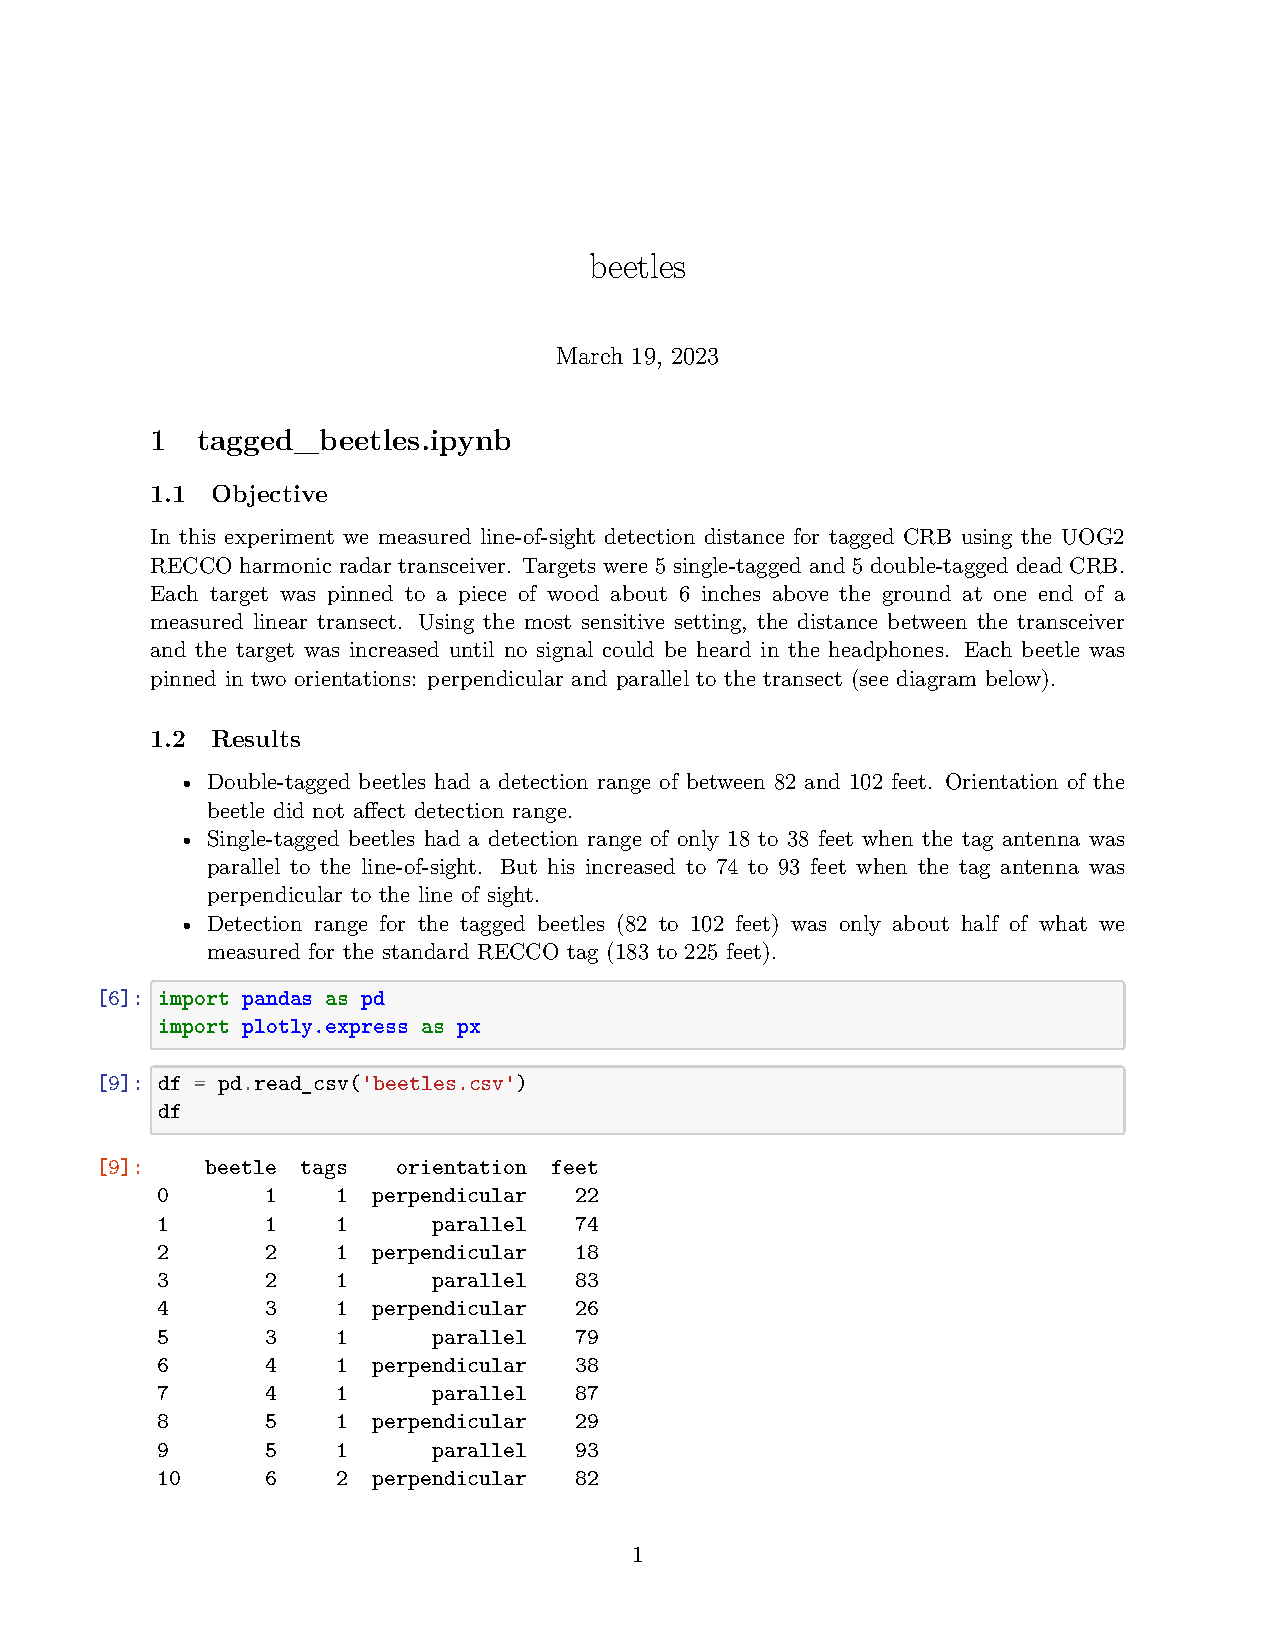
\includepdf[pages=-]{../experiments/detection-range/beetles.pdf}

\newpage
\section{Jupyter Notebook for Experiment 3: Attenuation of maximum detection distances when targets are buried in coir}
\label{exp3}
Please see next page.
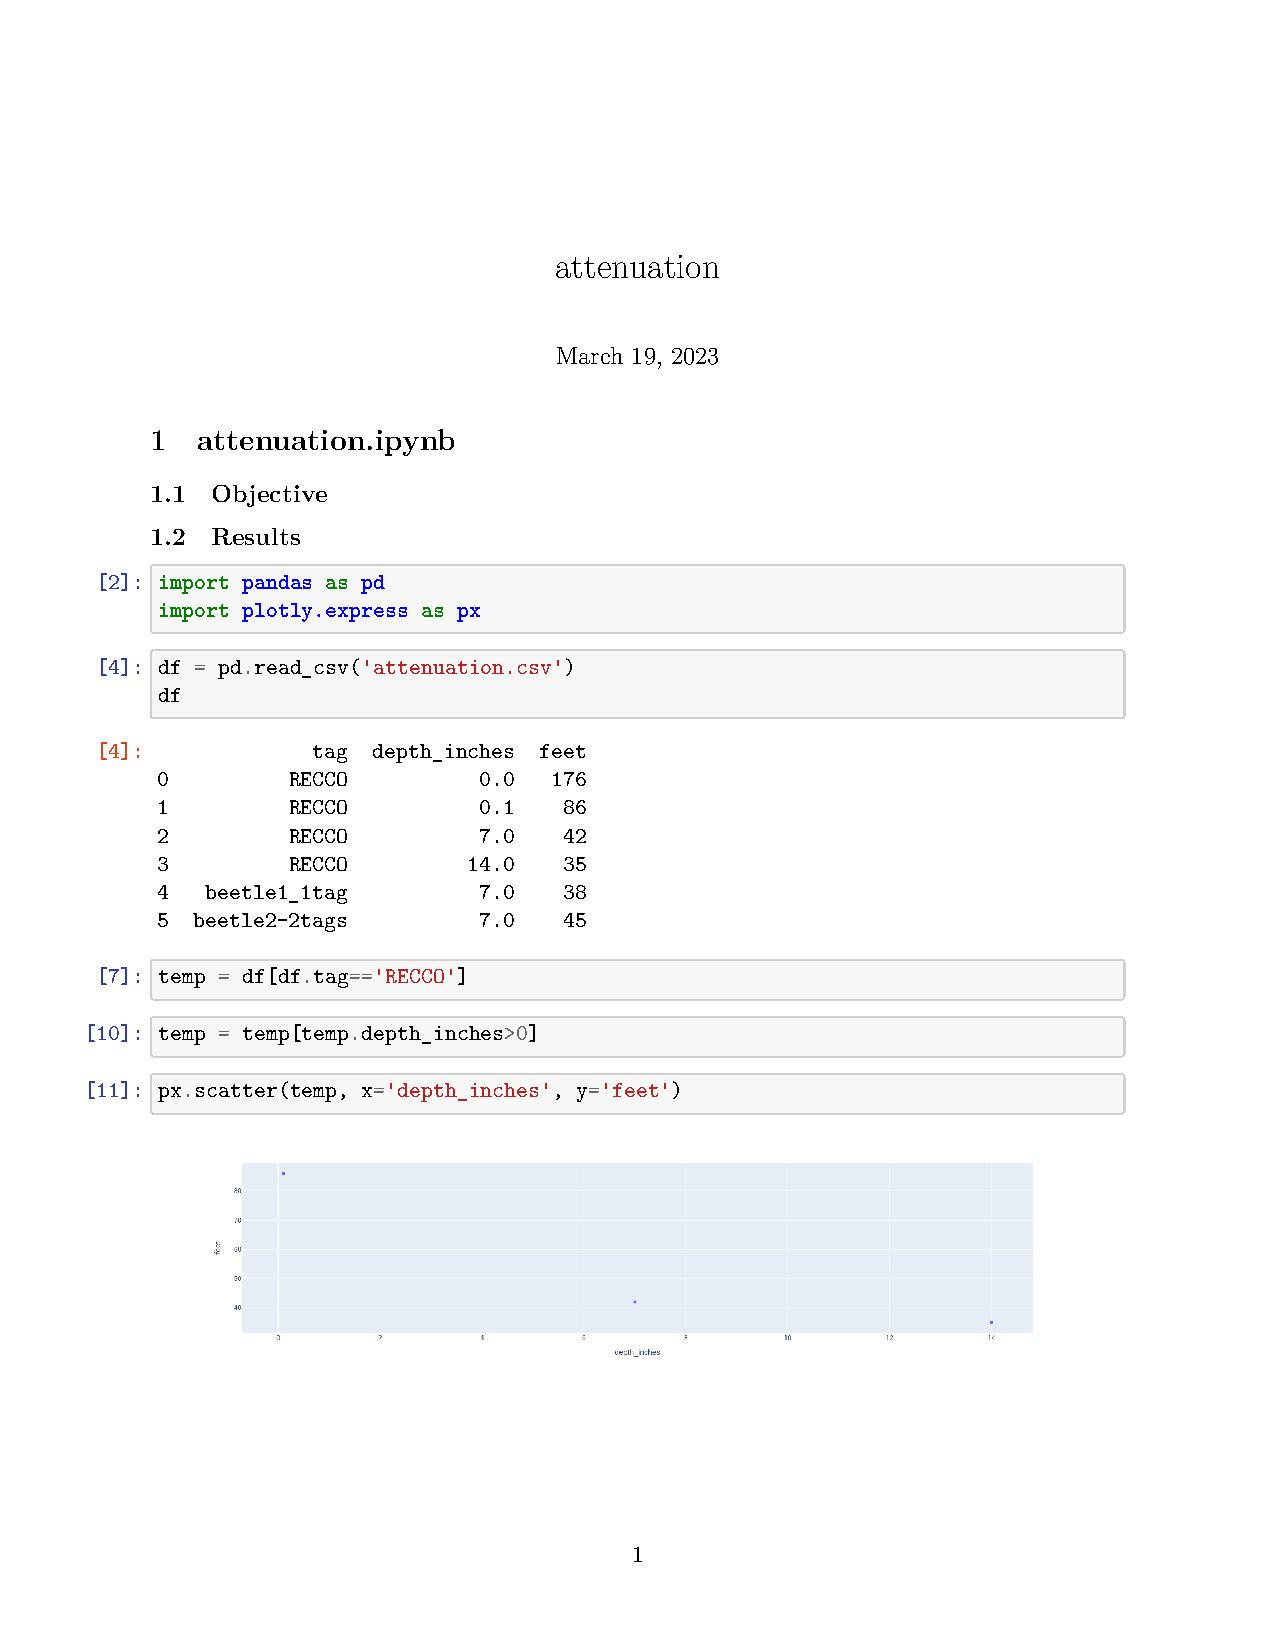
\includepdf[pages=-]{../experiments/detection-range/attenuation.pdf}

\end{appendices}

\end{document}
